\chapter{無線センサネットワーク}
\begin{large}
\begin{quote}
本章では,最初に無線センサネットワークの普及について説明する.
次に本研究の想定環境である,
環境モニタリングとターゲットトラッキングについてそれぞれ例を提示し,
%無線センサネットワークにおける,
エネルギーの節約とリアルタイム処理の必要性について述べる.
\end{quote}
\end{large}
\clearpage

\section{はじめに}
近年技術の発展によりセンサノードの低価格化,高性能化が進み,
それに伴い,ネットワークに繋がる物理センサが自動的に多様なデータをやり取りし,
それらを様々な形で活用する無線センサネットワークが普及してきている.
代表的なセンサノードとして,Iris MoteやMicaZ\cite{Hill:2002:MWP:623308.624560},
SunSPOTなどがある.

Iris Moteは図\ref{fig:iris_mote}のようなものであり,
アメリカのCrossbow Technology社が開発したセンサネットワーク用の無線端末である.
それに対して,MicaZはカリフォルニア大学バークレー校における
スマートダストプロジェクト\cite{Kahn:1999:NCC:313451.313558}によって開発された.
ハードウェア,オペレーティングシステム,開発言語,シミュレータ,
ライブラリといったアプリケーション開発環境を提供しており,
アプリケーション開発が容易であるため,
現在センサネットワークの研究で多く使用されている.
図\ref{fig:micaz}にMicaZの写真を示す.
MicaZは小型なため,様々な場所に応用することができる.
SunSPOTは図\ref{fig:sunspot}のようなものであり,
サン・マイクロシステムズが開発したIEEE 802.15.4に準拠した無線センサーネットワークデバイスである.
SunSPOTとはSun Small Programmable Object Technologyの略称であり,
Javaで実装することができるため,初心者でも扱いやすいセンサデバイスとなっている.


\begin{figure}[htbp]
 \begin{minipage}{0.5\hsize} \begin{center}
     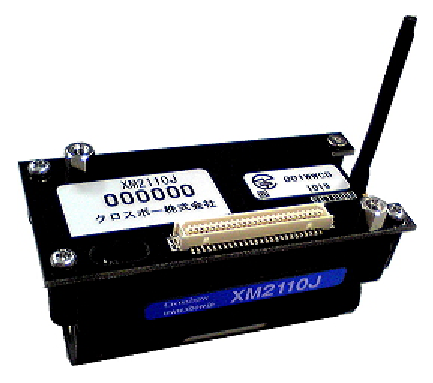
\includegraphics[width=40mm]{./images/iris_mote.eps}
    \end{center}
    \caption{Iris Mote}
    \label{fig:iris_mote}
 \end{minipage}
 \begin{minipage}{0.5\hsize}
    \begin{center}
     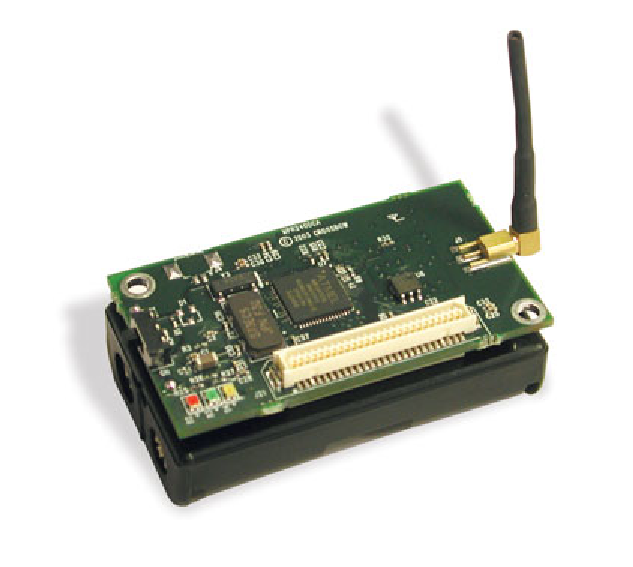
\includegraphics[width=45mm]{./images/micaz.eps}
    \end{center}
    \caption{MicaZ}
    \label{fig:micaz}
 \end{minipage}
\end{figure}

\begin{figure}[htbp]
 \begin{center}
  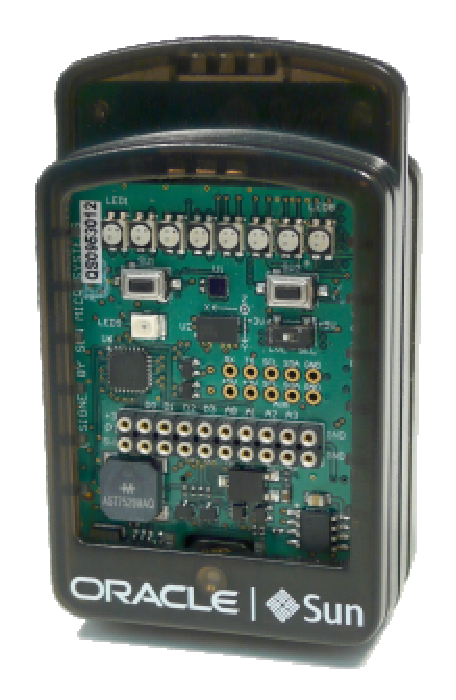
\includegraphics[width=25mm]{./images/sunspot.eps}
 \end{center}
 \caption{SunSPOT}
 \label{fig:sunspot}
\end{figure}





\section{環境モニタリング}
環境モニタリングの歴史は長く,
かつては手動によりデータの収集を行っていたが,
デジタルデータロガーの普及により,
より安く,容易にデータの授受を行うことができるようになった.
しかしながら,環境モニタリングでは大抵の場合,
対象となる範囲全域での監視が求められていることに対して,
デジタルデータロガーを利用した場合,
ある一点においてのみのモニタリングしか行うことができなかったため,
デジタルデータロガーに代わる
環境モニタリングの次なる手段として,
無線センサネットワークが採用され始めている.
センサノードには様々なセンサが搭載されており,
センサノードを対象とする地域に配置し,
ネットワークを構築することで,
デジタルデータロガーでは成し得なかった,
広範囲におけるモニタリングを可能としている.

無線センサネットワークを用いた環境モニタリングでは,
モニタリング対象の行動に変化があった際には,
それに応じたタスクを優先的に行わなければならない.
このような時間的制約を伴ったタスクの処理が必要なアプリケーションを想定した場合,
オペレーティングシステムとして
リアルタイム処理を行うことが可能なものを選択することが多い.
無線センサネットワークにおけるオペレーティングシステムのリアルタイム性については,
\ref{sec:threads_model}において詳細に述べる.
本節では代表的な環境モニタリングとして,
森林火災検知と野生動物の生態調査を例に挙げる.




\subsubsection{森林火災検知}

\vspace{0.5em}森林火災は原生林において生じる制御不可能な火災であり,
自然資源と人的資源に多大な被害を与える.
具体的に,木々を根絶やし,基盤となる施設を燃やし,
さらには都市部付近における死亡者数を増加させてしまう場合も少なくない.
森林火災の共通の原因として,落雷や人間の不注意,
そして燃料の野ざらしによる極度の乾燥などが挙げられる.
場合によっては火災は森林の生態系の一部としてみなされることもあるが,
ほとんどの場合において,
火災により発生する公衆安全や自然資源に対するダメージは耐え難いものであり,
被害を最小限に抑えるためにも火災の早期発見と鎮圧が極めて重要である.
%森林火災検知システムにおいて,
%災害の規模を最小化するために即座に対応することが最も重要であることは既に述べたが,
しかしながら低解像度かつ長期走査により,
%現在の
中規模もしくは大規模火災監視システムは適時検知を行うことは困難であり,
高精度のリアルタイム火災検知を提供できる拡張性のある手法が求められていた.

近年無線センサネットワークにおける発展が著しく,
森林火災を検知する際に役立つ,温度,相対湿度,さらに煙などの
様々な現象をセンシングすることが可能であることから,
無線センサネットワークがこれらの問題を解決できる手法として関心を集めている.
%リアルタイム森林検知システム構築するための将来有望なフレームワークを構築.
%近い将来,
%森林火災検知のための
%様々なセンシングモジュールが明確にデザインされ,
%最適化される.
%加えて,
火災が発生している間,定期的な監視を実現するために,
センサノードは数週間にわたってオペレーションをすることが可能であり,
%航空機を利用することで,
森林火災によって生じる被害と比較しても,
低コストで大規模センサネットワークは容易に展開することができる.


森林火災検知システムにおけるネットワークライフタイムは,
約6ヶ月から成る火災シーズンを少なくとも上回ることが望ましいが,
一般的にそれぞれのノードが数週間に渡って稼働することは難しいのが現状である.
したがってこの要件を満たすためにも,
エネルギーの消費を抑えるようなシステムを提案する必要がある.


森林火災モニタリングに対する無線センサネットワークの可能性について考察したDoolinらは,
サンフランシスコとカリフォルニアにおける制御下の火災から実験的な結果を導き出した
\cite{doi:10.1117/12.605655}.
システムはGPSを搭載した数個のMica Moteから成り,
収集された温度,湿度,そして気圧データはベースステーションへと転送され,
データベースへと格納後,異なるアプリケーションによって提供される
(図\ref{fig:system_conf_of_WS_for_wildfire_monitoring}).
実験から,火災発生地域多数のセンサを設置することで,
火災が発生するより前に火災発生の前触れを予測することができると述べている.

\begin{figure}[htbp]
 \begin{center}
  \includegraphics[width=100mm]{./images/system_conf_of_WS_for_wildfire_monitoring.eps}
 \end{center}
 \caption{無線センサを用いた森林火災モニタリングシステム構成図}
 \label{fig:system_conf_of_WS_for_wildfire_monitoring}
\end{figure}



また,森林火災の消火においては類焼を予測するために
温湿度の変化を観測することが重要であり,
これまでは消防士が測定器を持って位置時間ごとに測定を行っていたが,
この手法では消防司令所への報告に数分を要することに加え,
類焼する可能性のある危険な場所に消防士を向かわせなければならない.
森林火災を消火する消防士を支援するシステムである,
FireWxNet\cite{conf/mobisys/HartungHSH06}ではこのような温湿度の測定を,
無線センサネットワークとそのネットワーク間を
接続する長距離無線リンクで構成されるシステムを
利用して行うことを提案している(図\ref{fig:firewxnet_overview}).
実際にこのシステムを展開することで,
温湿度の測定結果や,データの通信成功率,バッテリ寿命について考察している.
局所的な測定をセンサネットワークで行い,
そのデータを長距離無線リンクで伝送することで,
より現実的な無線センサネットワークの展開ができるという結果を示している.

\begin{figure}[htbp]
 \begin{center}
  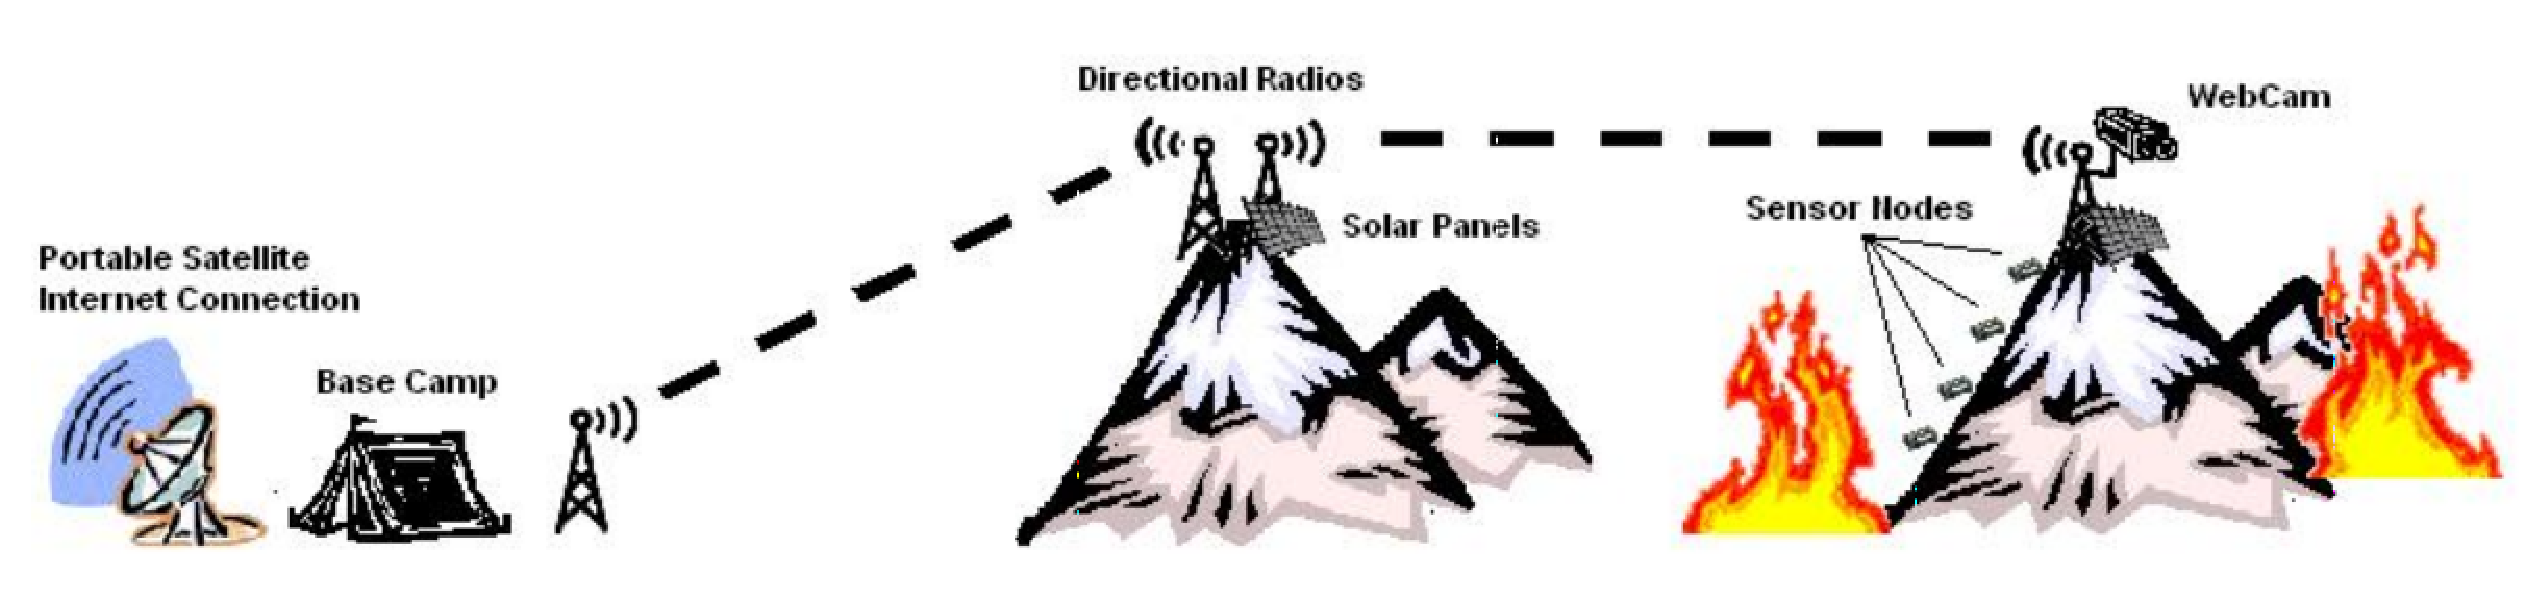
\includegraphics[width=140mm]{./images/firewxnet_overview.eps}
 \end{center}
 \caption{FireWxNet概要}
 \label{fig:firewxnet_overview}
\end{figure}




\subsubsection{野生動物の生態調査}

\vspace{0.5em}生命科学における研究者たちは
現地条件における動植物の観察する際に生じる,
人間という存在の潜在的影響について懸念を抱いていた.
近年,無線センサネットワークが既存の動植物の観察手法と異なる
手法のひとつとして注目されている.
動物の場合一般的にセンサは繁殖期のはじまりに前もって設置され,
植物の場合にはセンサの設置は地面が凍る,もしくは休眠状態にあるときに設置されるため,
動植物に与える影響が少なく,
繰り返し現地調査を行うことが困難であるような危険な島におけるモニタリングへの
負担も軽減できることから,
無線センサネットワークを基盤としたモニタリングは,
センサネットワークが普及する以前の弊害を無視した手法と比較して,
目覚ましい業績をあげている.
%Sensor networks represent a significant advance over traditional invasive methods of monitoring.
%Sensors can be deployed prior to the onset of the breeding season or other sensitive period (in the case of animals) or while plants are dormant or the ground is frozen (in the case of botanical studies). 
%Sensors can be deployed on small islets where it would be unsafe or unwise to repeatedly attempt field studies. 
%The results of wireless sensor-based monitoring efforts can be compared with previous studies that have tradition- ally ignored or discounted disturbance effects.

調査対象の特徴によっては,
現地調査を複数回行うことが困難となる場合があることは既に述べたが,
無線センサネットワークに用いられる小型デバイスにおける
バッテリの駆動時間は,一般的なラップトップなどと比較して
かなり短いのが現状である.
バッテリを交換する回数が増えるにつれ,
無線センサネットワークから得られる利益は減少してしまうことから,
火災検知システムと同様に,省エネルギーが実現できるような
システム構成が求められている.


カリフォルニア大学バークレー校とインテルの研究員により,
Mica Moteを基盤とした
ウミツバメの生態を観測するための
階層型センサネットワークがグレート・ダック島に展開された
\cite{Mainwaring:2002:WSN:570738.570751}.
システム構成図は図\ref{fig:gdi_system_architecture}の通りである.
動物の掘った穴など,注目すべき32箇所にMica Moteが設置され,
区画ごとにグループ化されたそれらのMoteは,
センサデータをゲートウェイまで転送し,
さらにローカルネットワークを通して,
ベースステーションまでデータを転送する.
その後,ベースステーションでデータを記録し,
定期的に複製されたデータはデータベースへと格納される.
ユーザはデータベースサーバ内の複製されたデータにアクセスすることや,
サンプリングレートや電力を操作する変数を調整するなどの,
インタラクションをするためのデバイスを利用することが可能である.

\begin{figure}[htbp]
 \begin{center}
  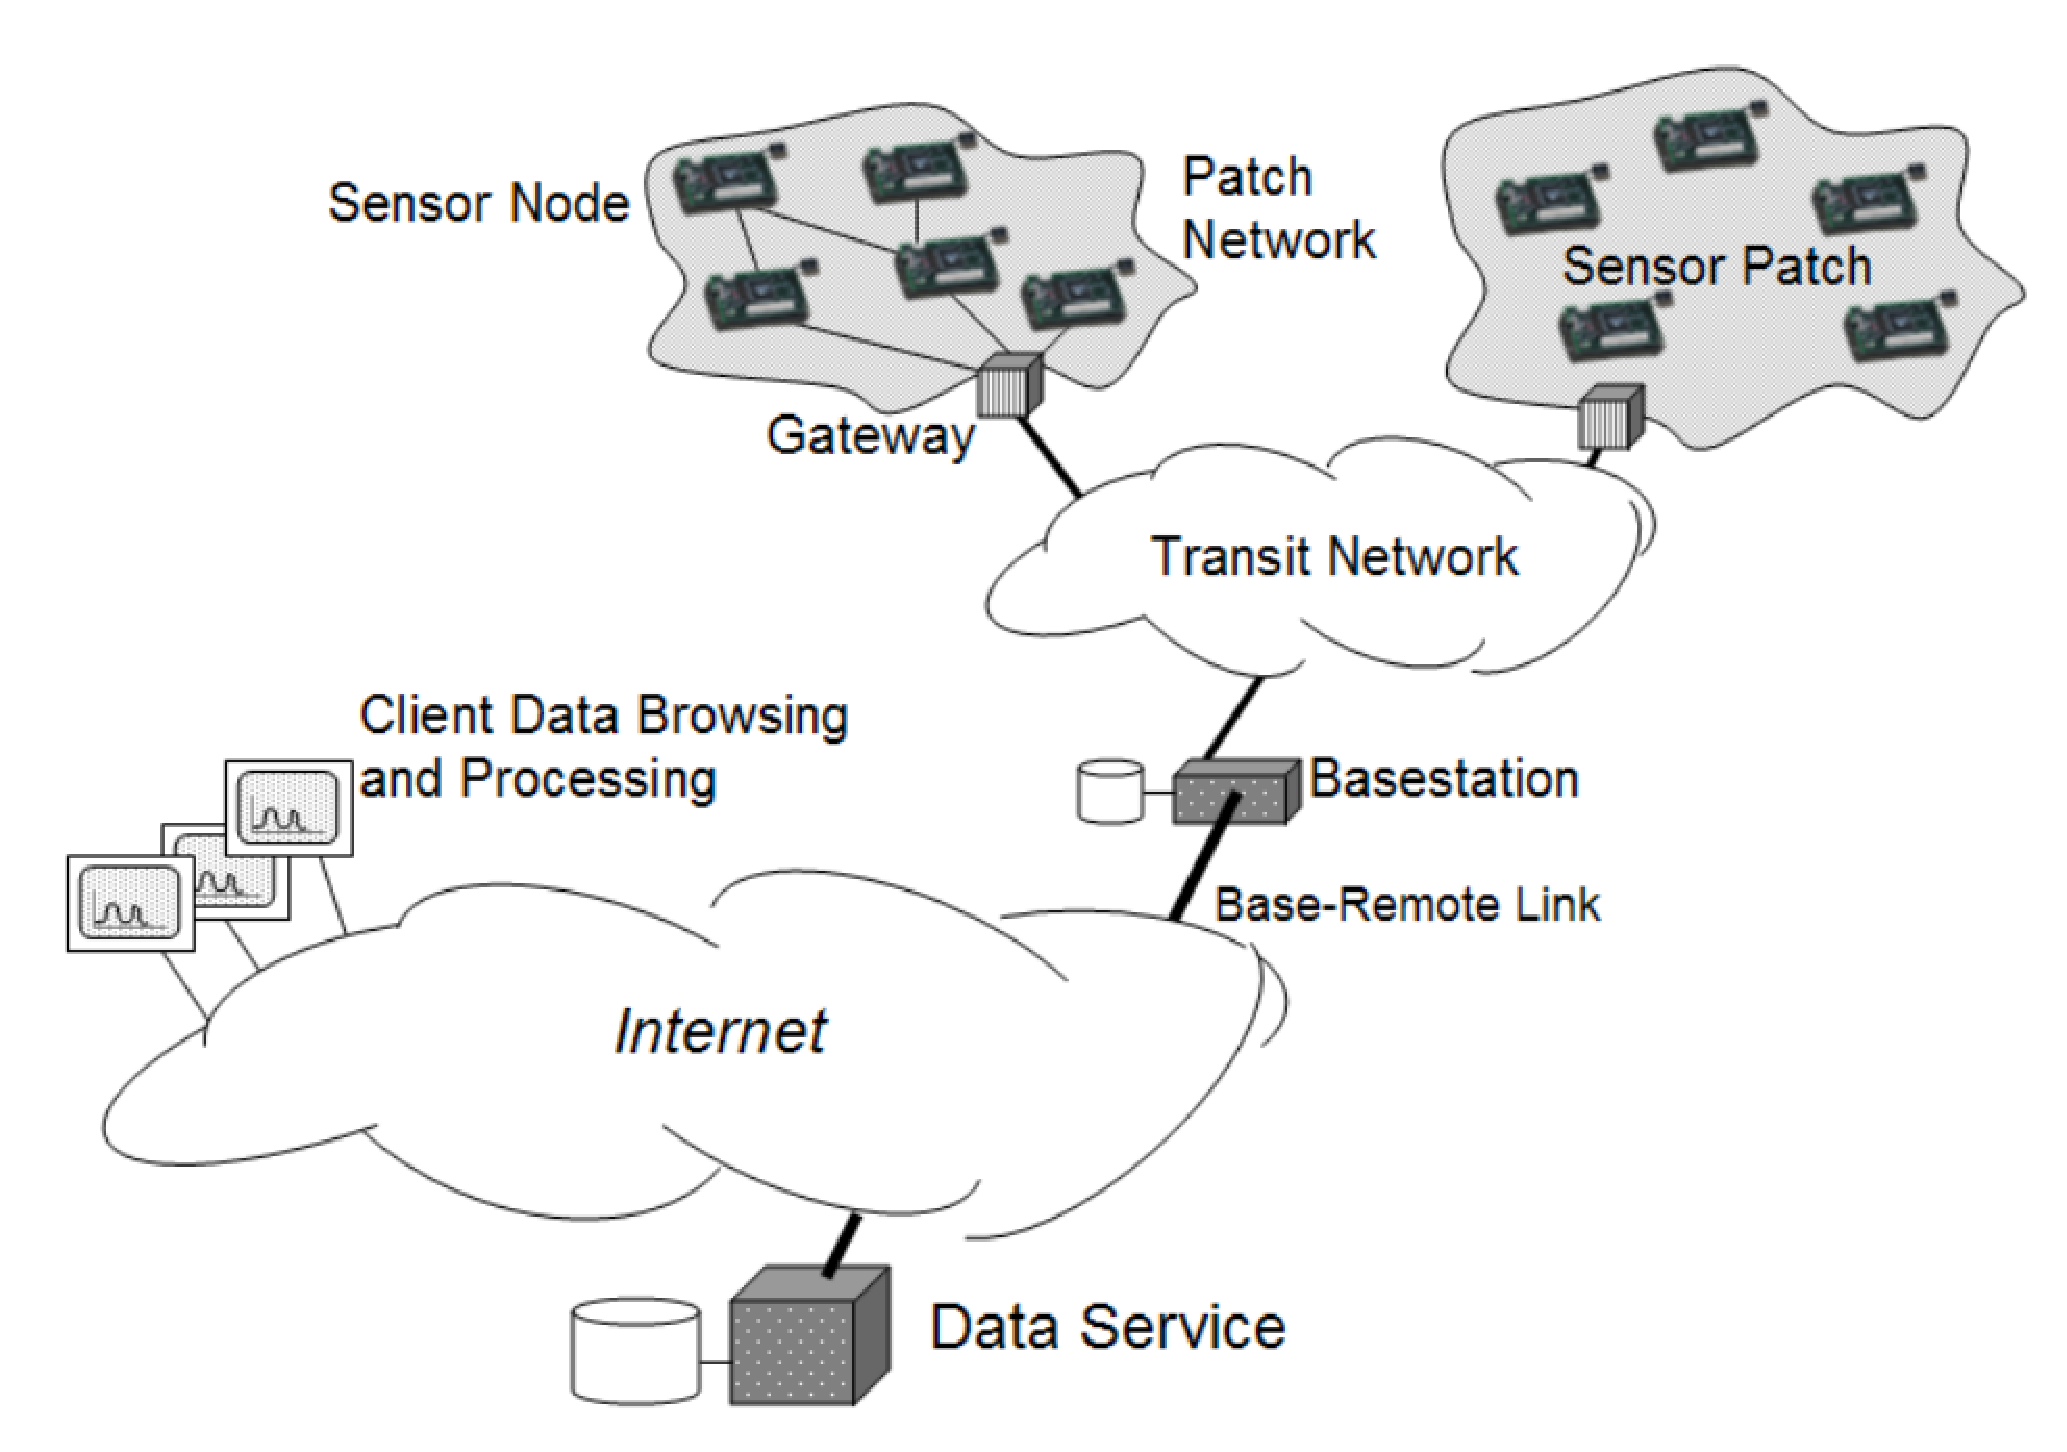
\includegraphics[width=120mm]{./images/gdi_system_architecture.eps}
 \end{center}
 \caption{GDIのシステム構成図}
 \label{fig:gdi_system_architecture}
\end{figure}




\section{ターゲットトラッキング}
%近年無線センサネットワークにおける,
%ターゲットトラッキングアプリケーション開発は
%ますます重要な位置づけになりつつある.
%Target Tracking as it moves through a sensor network has become an 
%increasingly important application in Wireless Sensor Networks. 

%物理環境において,
%特定のイベントの観測のための資源の限られた幾千ものセンサノードから成る,
%無線センサネットワーク技術に普及により,
%様々なシナリオにおける無線センサネットワークの利活用が
%現実的になりつつある.
%イベントを検知したセンサの周辺ノードはそのイベントを監視し,
%ラップトップやベースステーションのような外界と通信する機能を持った
%シンクノードに対してイベントの発生を知らせる.
%%The continuous evolution in wireless sensor network technology 
%%make it possible to implement the wireless sensor network (WSNs) in a variety of scenarios. 
%%WSNs consist of thousands of tiny sensor nodes deployed 
%%in a physical environment for observation of an event of interest. 
%%The sensors in the vicinity of an event must be able to monitor it and report back to the sink. 
%%A sink sensor node has capability to communicate with outside world such as laptop,base station. 
%
%
%近年,交通量管理や侵入者検知,野生動物の生態調査などの分野において,
%%センサノードは重要な役割を担っている.
%センサノードは重要な役割を担っている.
%無線センサネットワークにおける既存のターゲットトラッキングでは
%集約的な手法が用いられている.
%ネットワーク内におけるセンサの数が増加につれて,
%シンクノードに対するメッセージも増加し,
%それに伴い新たな帯域を消費してしまう.

%Sensor nodes have been deployed to play significant roles in traffic control,battlefield,
%habitat monitoring and intruder tracking in recent years. 
%The traditional target tracking methods for Wireless Sensor Networks 
%make use of a centralized approach. 
%As the number of sensors rise in the network,
%more messages are passed on towards the sink and will consume additional bandwidth. 
%Thus this approach is not fault tolerant 
%as there is single point of failure and lacks scalability. 
%Moreover in traditional target tracking methods,
%sensing task is usually performed by one node at a time resulting 
%in less accuracy and heavy computation burden on that node. 
%In WSNs each node has very limited power; 
%consequently traditional tracking methods 
%based on complex signal processing algorithms are not useful.

%物理環境において,
特定のイベントの観測のための資源の限られた幾千ものセンサノードから成る,
無線センサネットワーク技術に普及により,
様々なシナリオにおける無線センサネットワークの利活用が
現実的になりつつあることは既に述べたが,
交通量管理や侵入者検知などの
ターゲットトラッキングの分野は,
その影響が顕著に表れている分野のひとつである.

イベントを検知したセンサの周辺ノードはそのイベントを監視し,
ラップトップやベースステーションのような外界と通信する機能を持った
シンクノードに対してイベントの発生を知らせるのだが,
ターゲットトラッキングにおいて,
対象を検知し,その旨をシステムのゲートウェイノードに警告するタスクにより
中継されたデータは,
適時にゲートウェイまで届けられるべきである.
したがって,環境モニタリングと同様に
ターゲットトラッキングでもリアルタイムオペレーティングシステムを採用すべきである.
%このような時間的制約を伴ったデータの配送が必要なアプリケーションを想定した場合,
%オペレーティングシステムとして
%リアルタイム処理を行うことが可能なものを選択することが多い.
%無線センサネットワークにおけるオペレーティングシステムのリアルタイム性については,
%\ref{sec:threads_model}において詳細に述べる.
%ターゲットトラッキングアプリケーションにおいて,
%ある特定の時間にターゲットをセンシングしているセンサノードは
%アクティブモードを維持し,
%エネルギーを浪費しないように,
%残りのノードはターゲットが対象ノードに接近するまでの期間
%待機モードを継続する.
%この際,継続して移動するターゲットを監視するために,
%いくつかのセンサ郡は
%ターゲットが到着する少し前から
%アクティブモードにへと移行しなければならない.
%このアクティブなセンサ郡は
%移動するターゲットの速度に依存して変化し,
%クラスタのヘッドによってスケジューリングされる.
%ターゲットトラッキングを行う際には,
%エネルギーや帯域,オーバヘッドのような
%ネットワークリソース感のバランスを
%どのようにして保つかということに焦点が当てられている.
本節ではターゲットトラッキングの例として,
軍用監視システムについて言及する.

%In a target tracking application,
%the sensor nodes which can sense the target at a particular time are kept in active mode 
%while the remaining nodes are to be retained in inactive mode 
%so as to conserve energy until the target approaches them. 
%To continuously monitor mobile target,
%a group of sensors must be turned in active mode just before target reaches to them. 
%This group of active sensors varies depending on the velocity of moving target and schedule from cluster head. 
%Ultimately, target tracking in course of maintaining the balance 
%between network resources like energy, bandwidth, and overheads is challenging.


%もし無線センサネットワークが適切に利用された場合,
%軍用のアプリケーションにおける情報収集にて,
%人間の力を必要とする機会が減少していき,
%近い将来には,
%センサデバイスが低価格で大量生産され,
%実社会に高密度に備え付けられることが予測される.

\subsubsection{軍用監視システム}

\vspace{0.5em}監視任務において,
ターゲットとする敵の能力や位置に関する情報を
正確に入手することが何よりも重要であるが,
そのような任務には隊員の危険を伴うものが多い.
無線センサネットワークを利用することで,
リスクを最小限に抑えつつ,
敵の侵入に関する情報を的確に把握する研究が盛んに行われている.
図\ref{fig:surveillance_system}は軍用監視システムにおける概念図である.

\begin{figure}[htbp]
 \begin{center}
  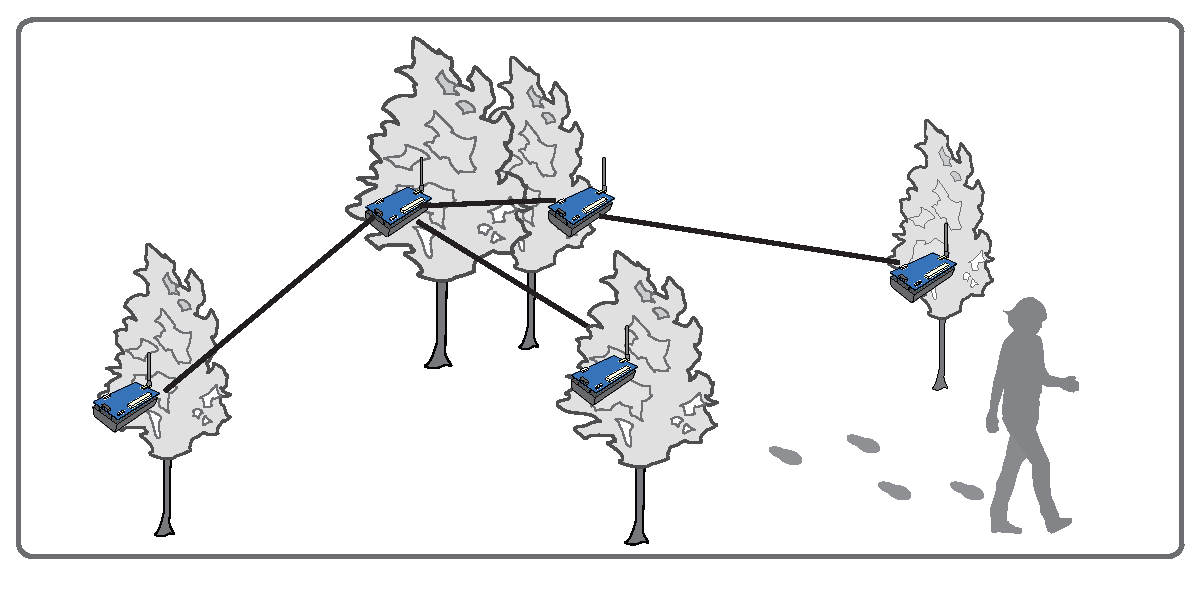
\includegraphics[width=100mm]{./images/surveillance_system.eps}
 \end{center}
 %\caption{イベント検知アプリケーション}
 %\caption{ターゲットトラッキングアプリケーション}
 \caption{軍用監視アプリケーションにおける概念図}
 \label{fig:surveillance_system}
\end{figure}


%監視アプリケーションにおいて,
%侵入者を検知し,その旨をシステムのゲートウェイノードに警告するタスクにより
%中継されたデータは,
%適時にゲートウェイまで届けられるべきである.
%上記のような時間的制約を伴ったデータの配送が必要なアプリケーションを想定した場合,
%オペレーティングシステムとして
%リアルタイム処理を行うことが可能なものを選択することが多い.
%無線センサネットワークにおけるオペレーティングシステムのリアルタイム性については,
%\ref{sec:threads_model}において詳細に述べる.

監視システムアプリケーションを用いた任務は
数日から数ヶ月にかけて行われるものが一般的であり,
任務中の秘密保持の重大性や
任務が敵の管轄地域行われる場合もあることから,
%近づきにくさ
任務期間中に資源の制限されたセンサデバイスの手動による充電はできないことがほとんどである.
したがって任務期間中継続して使用するために,
監視システムにおけるアプリケーションでは
センサデバイスの寿命を向上させるような
省エネルギーな構成が必要とされる.

また軍用の監視システムにおいて,
デイバイスが発見され,
それに伴い迎撃されることを
未然に防ぐことは極めて重要である.
センサデバイスを小型化することにより,
デバイスの発見を物理的に困難にすることができるが,
もしセンサデバイスが監視をする際に活発に通信をする場合,
無線周波数が傍受されてしまう可能性が高い.
重要なイベントが発生したときを除いて,
通信を控えることが求められている.

近年提案されている監視システムのほとんどが
シミュレーションを通して期待できる成果を挙げているが,
シミュレータを利用して単純化された仮説は
実環境において意図した通りの結果を得られないこともしばしばである.
Tian Heらの研究\cite{He04energy-efficientsurveillance}では,
省エネルギーかつステルス性を保ちながら移動する車両の位置を検知し,
追跡するセンサデバイスを用いた監視システムの設計と実装をし,
実空間においてシステムの感度を適宜調整することによって,
省エネルギー性と監視システムの性能におけるトレードオフについて考察している.
またこれに加えて,同期型の通信プロトコルを設計し,常にビーコンを送信し,
イベントが発生した場合はビーコンの送信を停止するProactive型と,
イベントが発生した場合にビーコンを送信するReactive型の実装を行い,
それぞれについて省電力性やステルス性などの評価も行っている.


%今日,充電不可能なバッテリを用いた数ヶ月間稼働するセンサネットワークに対する
%関心が高まっている.




%Sensor networks that run for 9 months from non-rechargeable power sources would have significant audiences today. 
%Although ecological studies at GDI span multiple field seasons,
%individual field seasons typically vary from 9 to 12 months. 
%Seasonal changes as well as the plants and animals of interest determine their durations.




%\section{イベント検知アプリケーション}

\section{まとめ}
本章では,最初にハードウェアに関する技術の発展から,
センサの小型化,高性能化が進み,
それに伴い無線センサネットワークが普及してきたことを説明した.
次いで,無線センサネットワークが適用されてきた一例として,
環境モニタリングとターゲットトラッキングを紹介し,
それぞれについてエネルギー節約とリアルタイム処理の重要性について言及した.

